\section{Auswertung}
\label{sec:Auswertung}
Für die Temperatur wurde eine Messunsicherheit von $\symup{\Delta} T = 0.1$ angenommen.
\subsection{Statisches Vefahren}  
\subsubsection{Vergleich der Temperaturverläufe}
\begin{figure}
  \begin{subfigure}{0.48\textwidth}
    \centering
    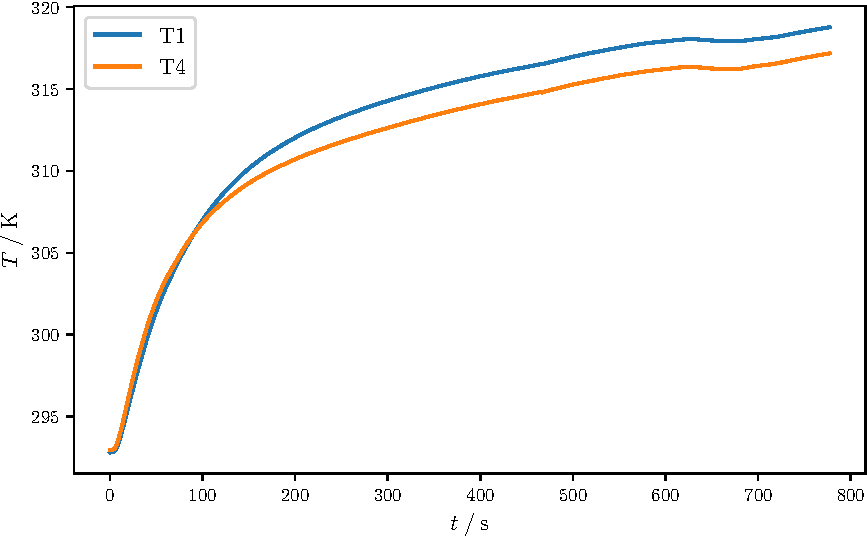
\includegraphics[width = \textwidth]{build/stat14.pdf}
    \caption{Temperaturverlauf $T_1$ und $T_4$}
    \label{fig:stat14}
  \end{subfigure}
  \begin{subfigure}{0.48\textwidth}
    \centering
    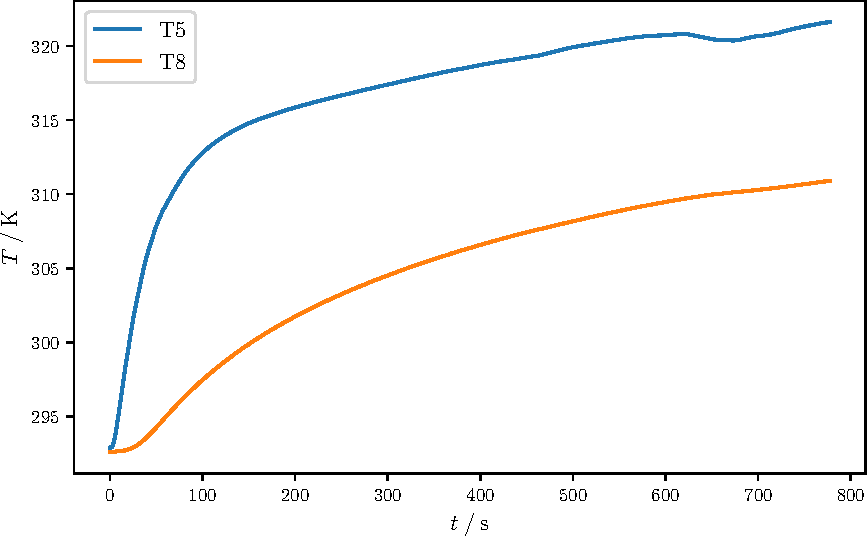
\includegraphics[width = \textwidth]{build/stat58.pdf}
    \caption{Temperaturverlauf $T_5$ und $T_8$}
    \label{fig:stat58}
  \end{subfigure}
\end{figure}
Bei dem Verglichen der Kurven fällt es auf, dass alle vier Kurven zu Beginn einen starken Temperaturanstieg repräsentieren, welcher jedoch schnell wieder abschwächt.
Dennoch verhalten sich die Temperaturen $T_1$ und $T_4$ Anfangs beinahe identisch, wobei die Temperaturen $T_5$ und $T_8$ dort Diskrepanzen aufzeigen. $T_5$ steigt 
sehr stark an und flacht vergleichsweise schnell wieder ab, während die Temperatur $T_8$ eine eher verhaltene Steigung aufweist, denn diese steigt sehr langsam an, besitzt
im Gegenzug daszu keinen abrupten Steigungsverlust. Nach dem beinahe identischen Verhalten, fällt die Kurve von $T_4$ früher ab, wonach dann eine kleine, annähernd konstante
Differenz zwischen den beiden Temperaturen herrscht. Aufgrund der verhaltenen Steigung der Temperaturkurve von $T_8$ ist die Differenz zwischen den beiden Kurven aus der 
Graphik \eqref{fig:stat58} schon von Anfang an sehr groß, wobei sich diese ab dem Zeitpunkt $t \approx \SI{150}{\second}$ eingestellt hat. Als letzte Gemeinsamkeit erkennt man leicht, dass
alle Kurven einen leichten Abfall bei $t \approx \SI{620}{\second}$ erleiden.
\subsubsection{Die beste Wärmeleitfähigkeit}
\begin{table}
  \centering
  \label{tab:Waeremleitfaehigkeit}
  \caption{Temperaturen nach $\SI{700}{\second}$}
  \sisetup{table-format = 3.2}
  \begin{tabular}{S S S S}
     \toprule
     {$T_1 \mathbin{/} \si{\kelvin}$} & {$T_4 \mathbin{/} \si{\kelvin}$} & {$T_5 \mathbin{/} \si{\kelvin}$} & {$T_8 \mathbin{/} \si{\kelvin}$}  \\
     \midrule
     318.06 & 316.42 & 320.66 & 310.28 \\
      \bottomrule
  \end{tabular}
\end{table}
Wie man anhand der Tabelle \eqref{tab:Waeremleitfaehigkeit} erkennen kann, hat Aluminium die beste Leitfähigkeit.
\subsubsection{Wärmestrom}
Für die Berechnung des Wärmestroms dient die Gleichung \eqref{eqn:Wärmemenge}. Jedoch lässt sich in diesem Fall die Wärmestromdichte
$j_w$ nicht mit dem Differntialquotient $\frac{\partial T}{\partial x}$ sondern "nur" mit dem Differenzenquotienten $\frac{\symup{\Delta}T}{\symup{\Delta} x}$
berechnen. Für den Abstand zwischen zwei Thermoelementen  wurde $\symup{\Delta} x = \SI{0.03}{\meter}$ gemessen.

\begin{table}
  \centering
  \caption{Ergebnisse der Differentialquotienten}
  \label{tab:Differentialquotient}
  \sisetup{table-format = 1.4}
  \begin{tabular}{S[table-format = 3.0] 
    S[table-format = 1.2] @{${}\pm{}$} S[table-format = 0.2] 
    S[table-format = 1.2] @{${}\pm{}$} S[table-format = 0.2] 
    S[table-format = 1.2] @{${}\pm{}$} S[table-format = 0.2] 
    S[table-format = 1.2] @{${}\pm{}$} S[table-format = 0.2]}
    \toprule
    {$t \mathbin{/} \si{\second}$} 
    & \multicolumn{2}{c}{$\frac{\symup{\Delta} Q_\text{M}}    {\symup{\Delta}t} \mathbin{/} \si{\joule\second\tothe{-1}}$}
    & \multicolumn{2}{c}{$\frac{\symup{\Delta} Q_\text{M, k}} {\symup{\Delta}t} \mathbin{/} \si{\joule\second\tothe{-1}}$}  
    & \multicolumn{2}{c}{$\frac{\symup{\Delta} Q_\text{A}}    {\symup{\Delta}t} \mathbin{/} \si{\joule\second\tothe{-1}}$}
    & \multicolumn{2}{c}{$\frac{\symup{\Delta} Q_\text{E}}    {\symup{\Delta}t} \mathbin{/} \si{\joule\second\tothe{-1}}$}\\
    \cmidrule(lr){2-3} \cmidrule(lr){4-5} \cmidrule(lr){6-7} \cmidrule(lr){8-9}
    \midrule
    600  & 16.42 & 0.10 & -10.07 & 0.13 & 0.10 & 0.10& 0.10 & 0.10\\
    900  & 14.48 & 0.12 & -9.50  & 0.16 & 0.12 & 0.12& 0.12 & 0.12 \\
    1200 & 12.55 & 0.13 & -8.93  & 0.20 & 0.13 & 0.13& 0.13 & 0.13\\
    2100 & 67.56 & 0.19 & -7.22  & 0.31 & 0.19 & 0.19& 0.19 & 0.19\\
    \bottomrule
  \end{tabular}
\end{table}